\textbf{Problem definition}:
Consider

%
\begin{equation}\label{eq:Q2}
	\dot{x} = x^3 + \delta x^2 - \mu x
\end{equation}
%

Determine the fixed points of the system and study the biforcations in the $(x, \mu)$ plane for non-zero values of $\delta$

\noindent\hrulefill

% -------------------------------------------------------------------
\textbf{Solution approach:} The stationary points are calculated by setting $\dot{x}$ equal to zero.

%
\begin{subequations}\label{eq:stationaryPoints}
\begin{align}2
	x &= 0 \label{eq:stationary0}
	\\
	x &= \frac{-\delta \pm \sqrt{\delta^2 + 4 \mu}}{2} \label{eq:stationary1}
\end{align}
\end{subequations}
%

The Jacobian for Equation \eqref{eq:Q2} is calculated as

%
\begin{equation}\label{eq:jacobian}
	D_x F = 3x^2 + 2 \delta x - \mu
\end{equation}
%

where $F = x^3 + \delta x^2 - \mu x$. The eigenvalue is written as

%
\begin{equation}\label{eq:eigenvalue}
	\lambda = 3x^2 + 2 \delta x - \mu
\end{equation}
%

The derivative of the forcing function to the control parameter, $\mu$, is calculated as:

%
\begin{equation}
	F_\mu = -x
\end{equation}
%

For $(x, \mu) = (0, 0)$ we have the following conditions:

%
\begin{equation}
\begin{cases}
	F(0, 0) = 0 \\
	D_x F \text{ has zero eigenvalue}
\end{cases}
\end{equation}
%

Therefore, we have satisfied the necessary conditions for the bifurcations. Since $F_\mu$ is in the range of $D_x F$ at $(0,0)$, we have a pitch fork bifurcation.

The bifurcation diagrams for various values of $\delta$ are shown in Figure \ref{fig:bifurcation}. In these plots, the dashed line represents the \emph{unstable branch} and the solid line represents the \emph{stable branch}. To calculate the turning point of the bifurcation diagram, we need to calculate the derivative of control variable, $\mu$, with respect to $x$ and set it equal to zero.

%
\begin{equation}
	x = \frac{-\delta \pm \sqrt{\delta^2 + 4 \mu}}{2} \Rightarrow
	\frac{d \mu}{dx} = \delta + 2 x
\end{equation}
% 

Therefore, the turning point is at $(-\dfrac{\delta}{2}, -\dfrac{\delta^2}{4})$. This can also be seen in Figure \ref{fig:bifurcation}.

%
\begin{figure}[h]
	\centering
	\begin{subfigure}[h]{8.0 cm}
		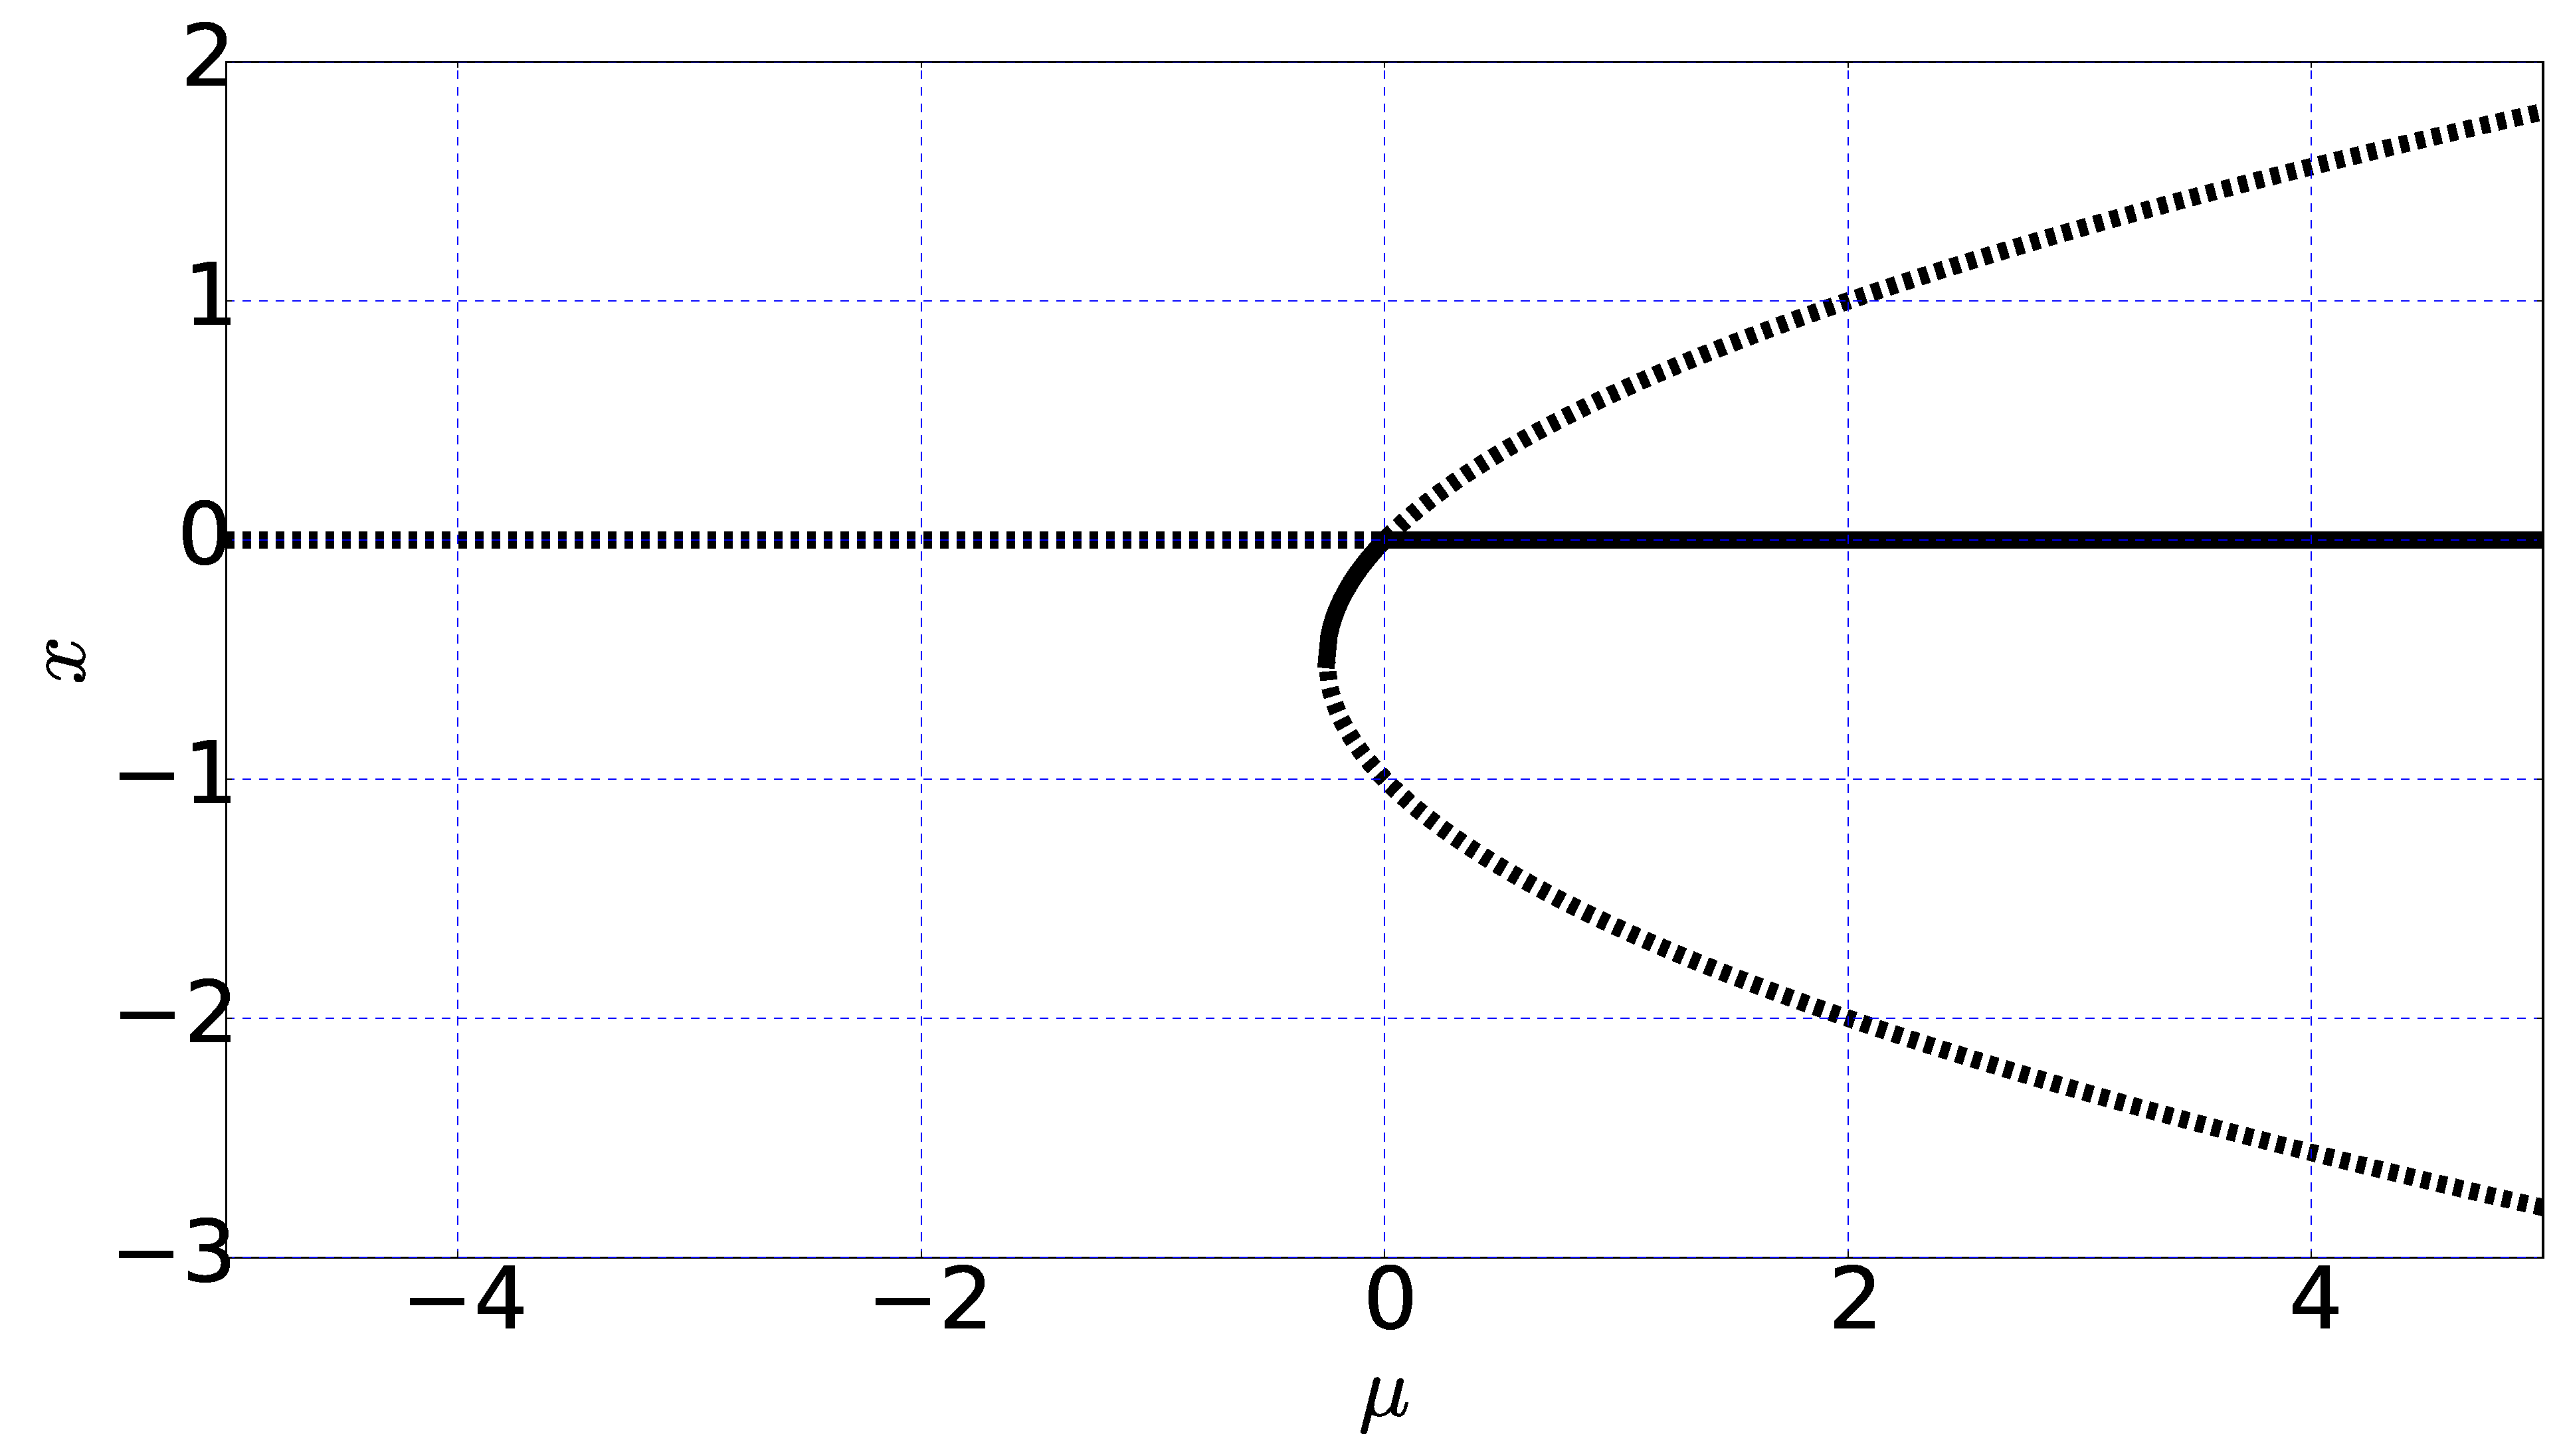
\includegraphics[width=8.0 cm]{figure/Q2/modified/delta1.eps}
		\caption{$\delta = 1$}
	\end{subfigure}
	\begin{subfigure}[h]{8.0 cm}
        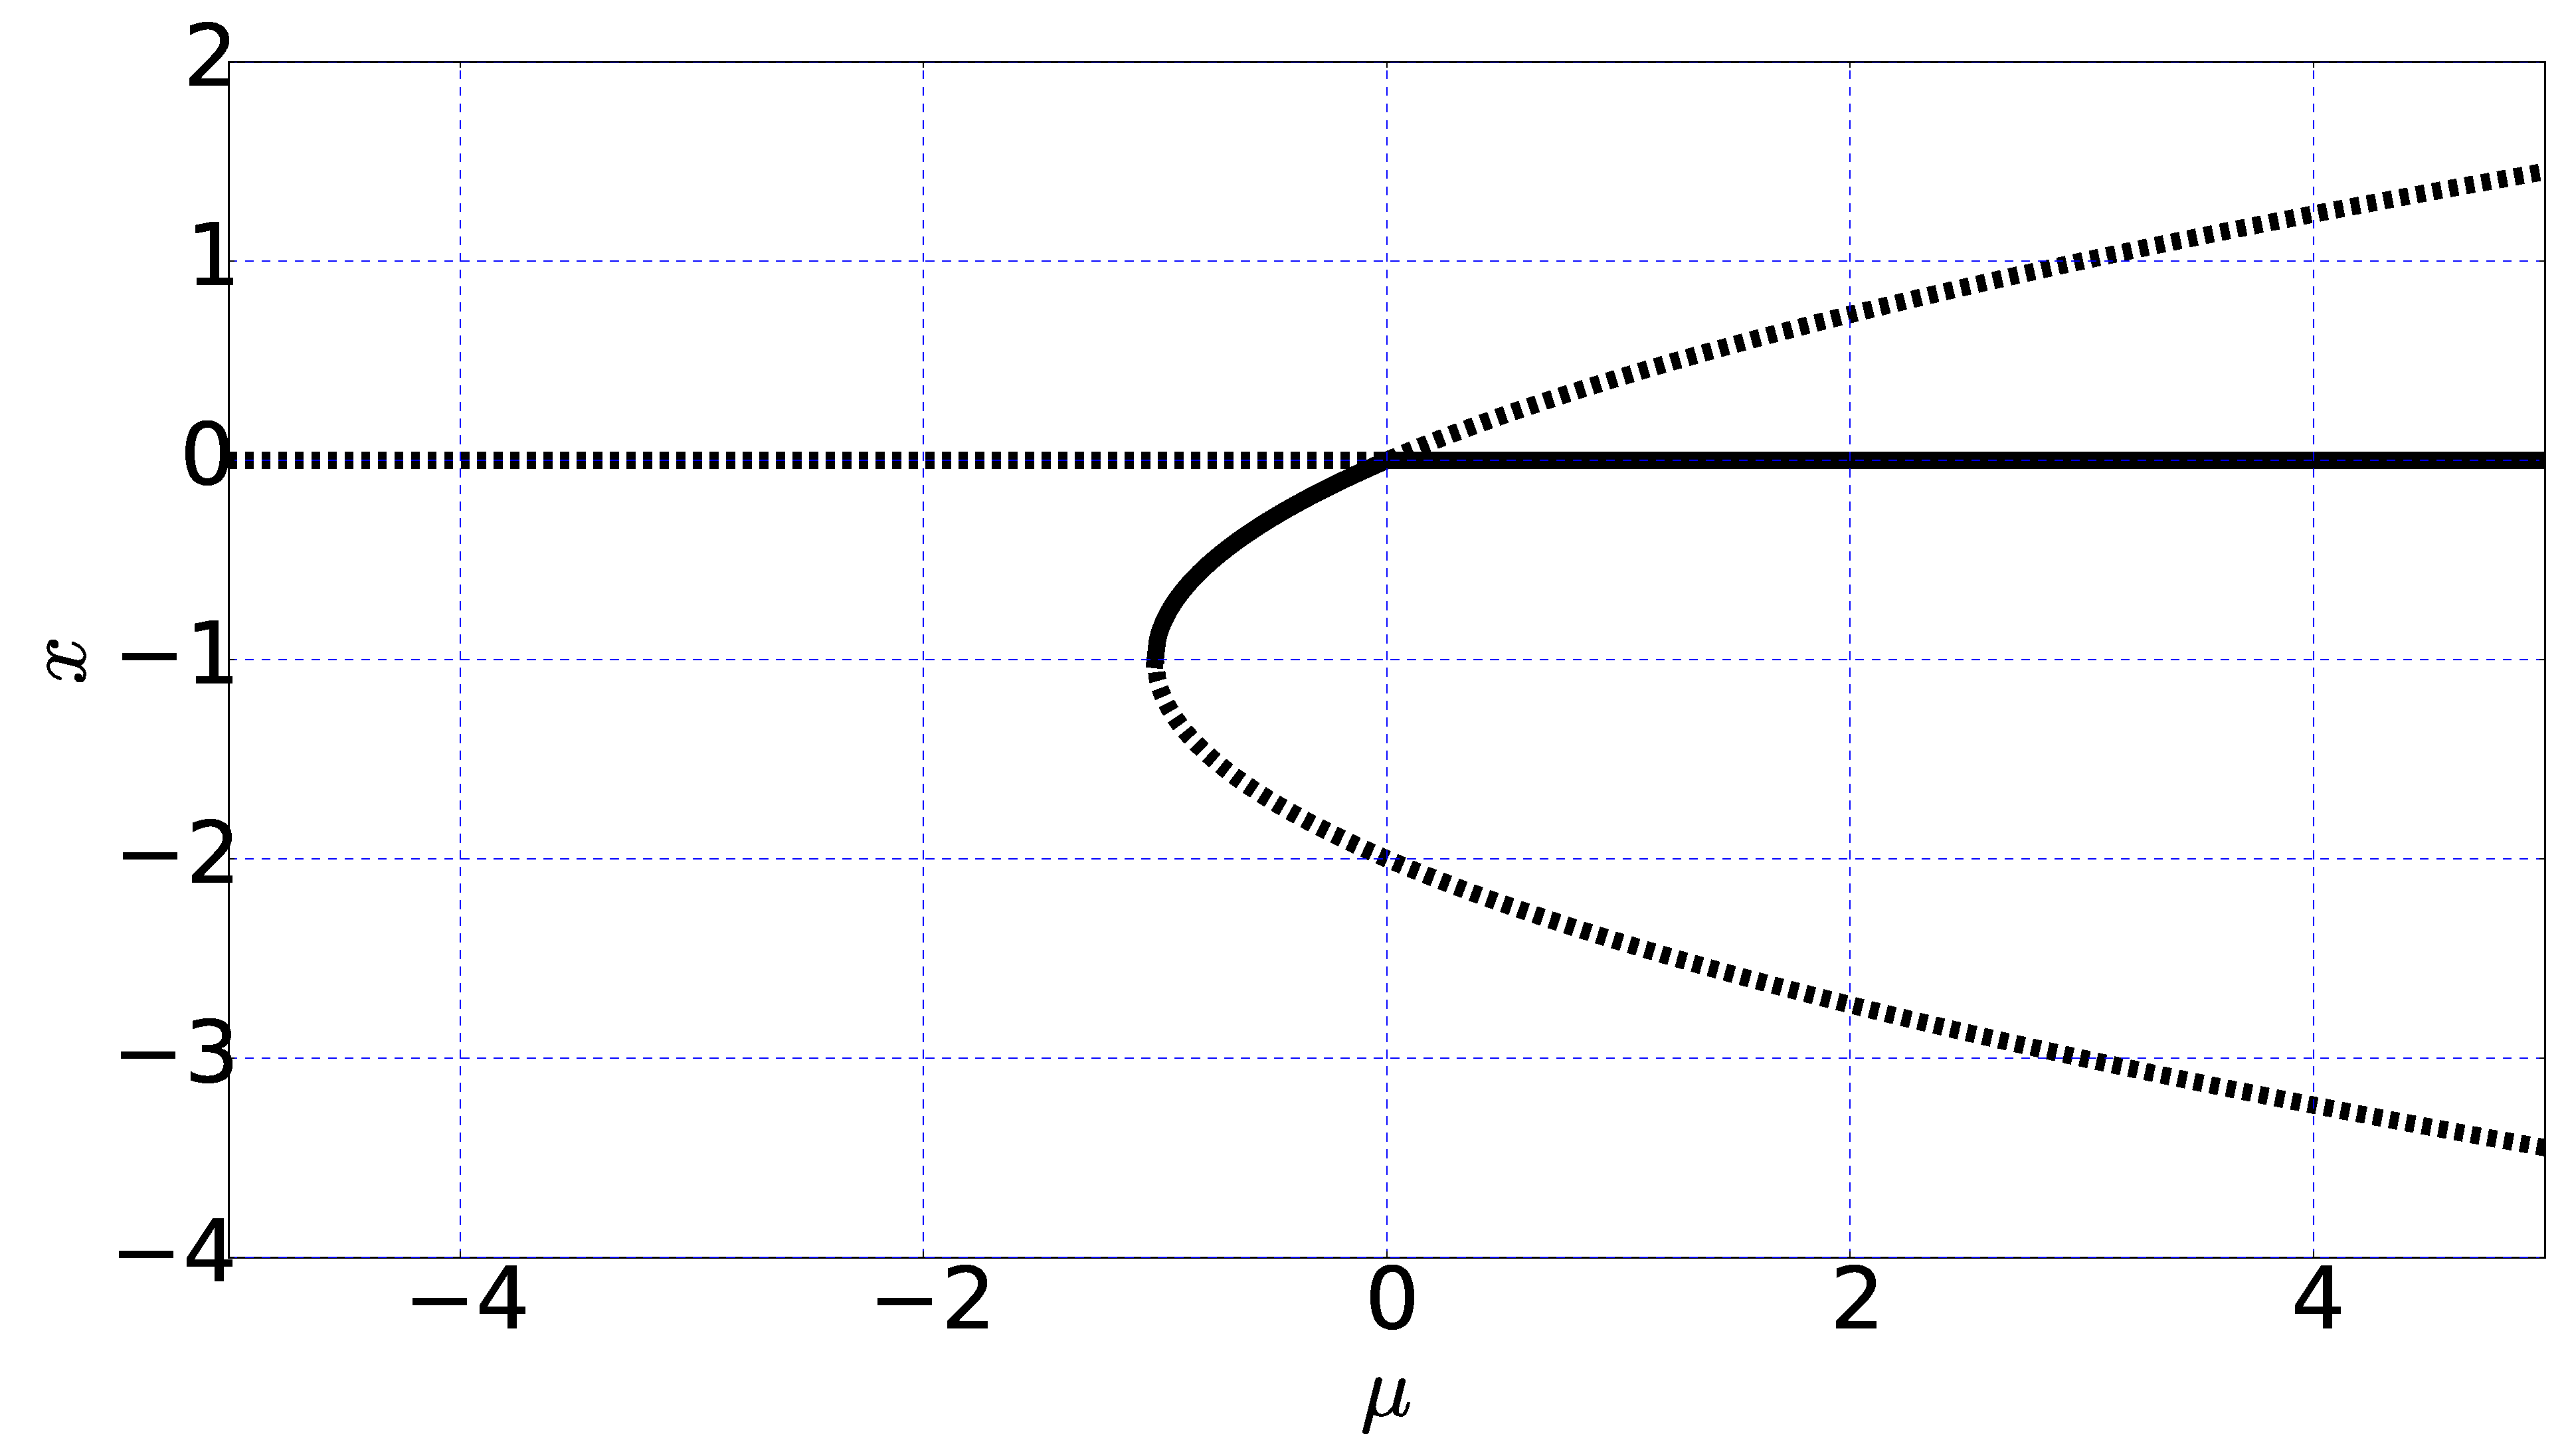
\includegraphics[width=8.0 cm]{figure/Q2/modified/delta2.eps}
		\caption{$\delta = 2$}
    \end{subfigure}
    \\
    \begin{subfigure}[h]{8.0 cm}
		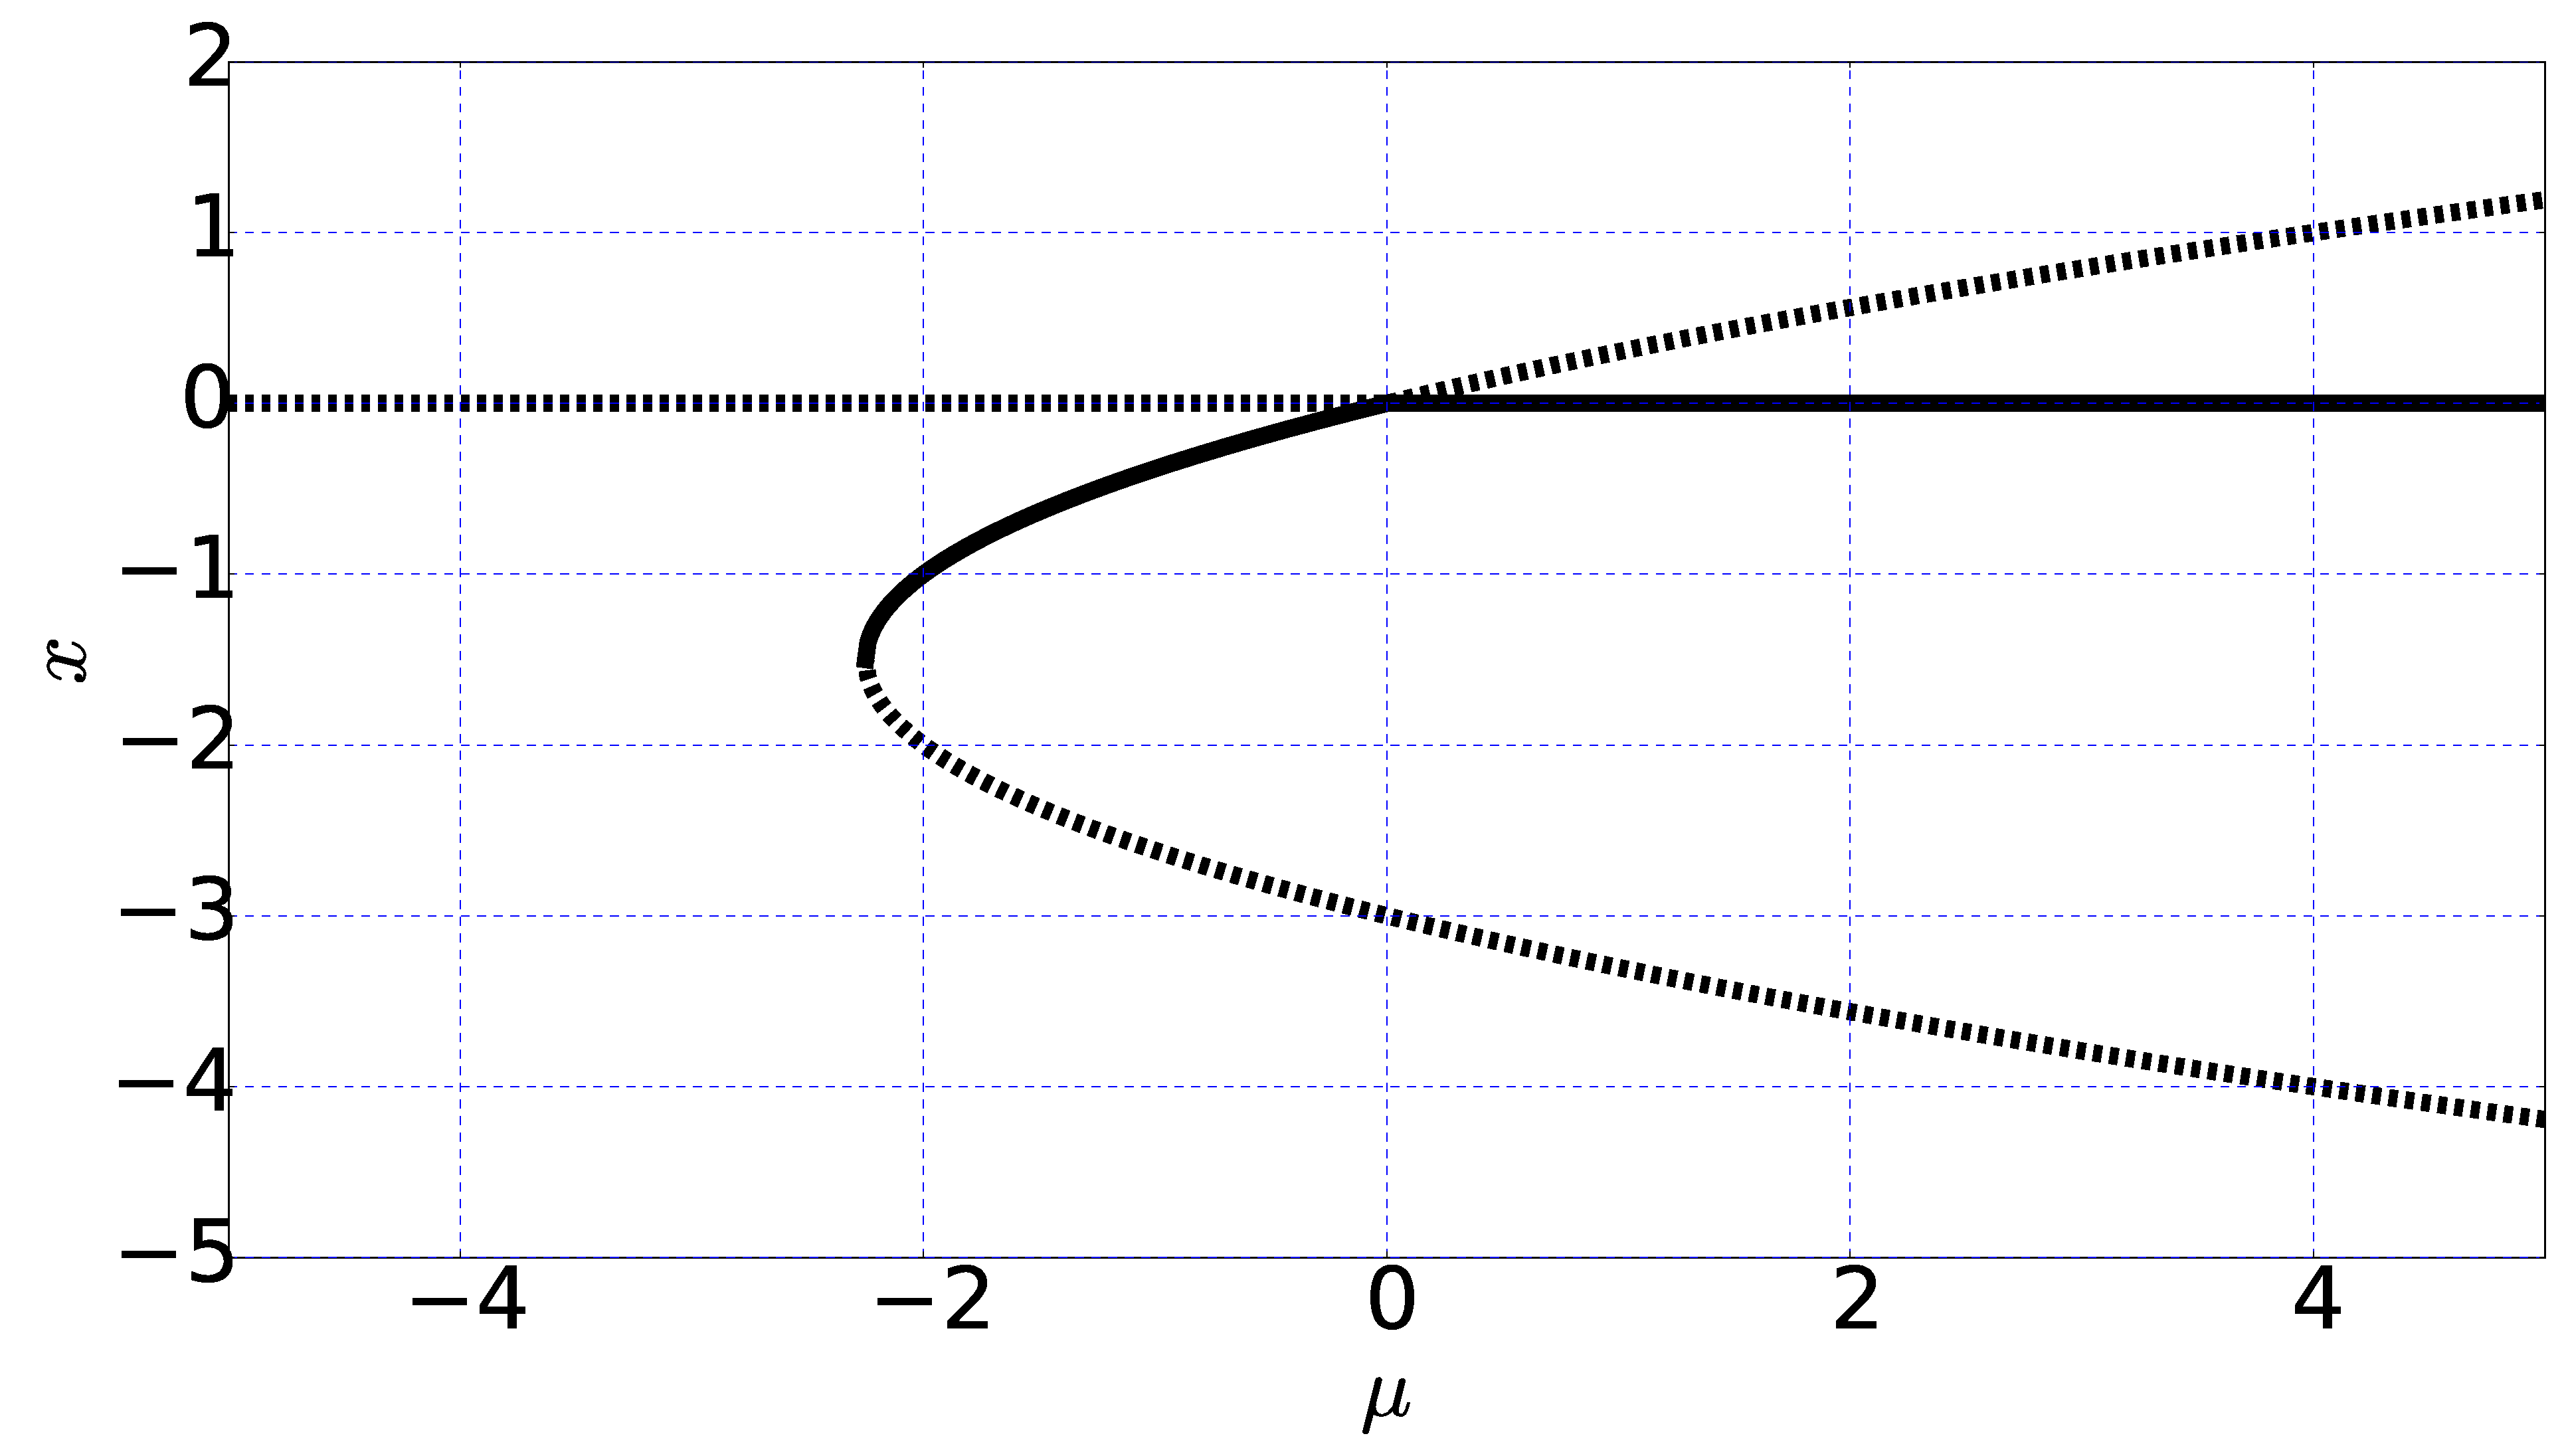
\includegraphics[width=8.0 cm]{figure/Q2/modified/delta3.eps}
		\caption{$\delta = 3$}
	\end{subfigure}
	\begin{subfigure}[h]{8.0 cm}
        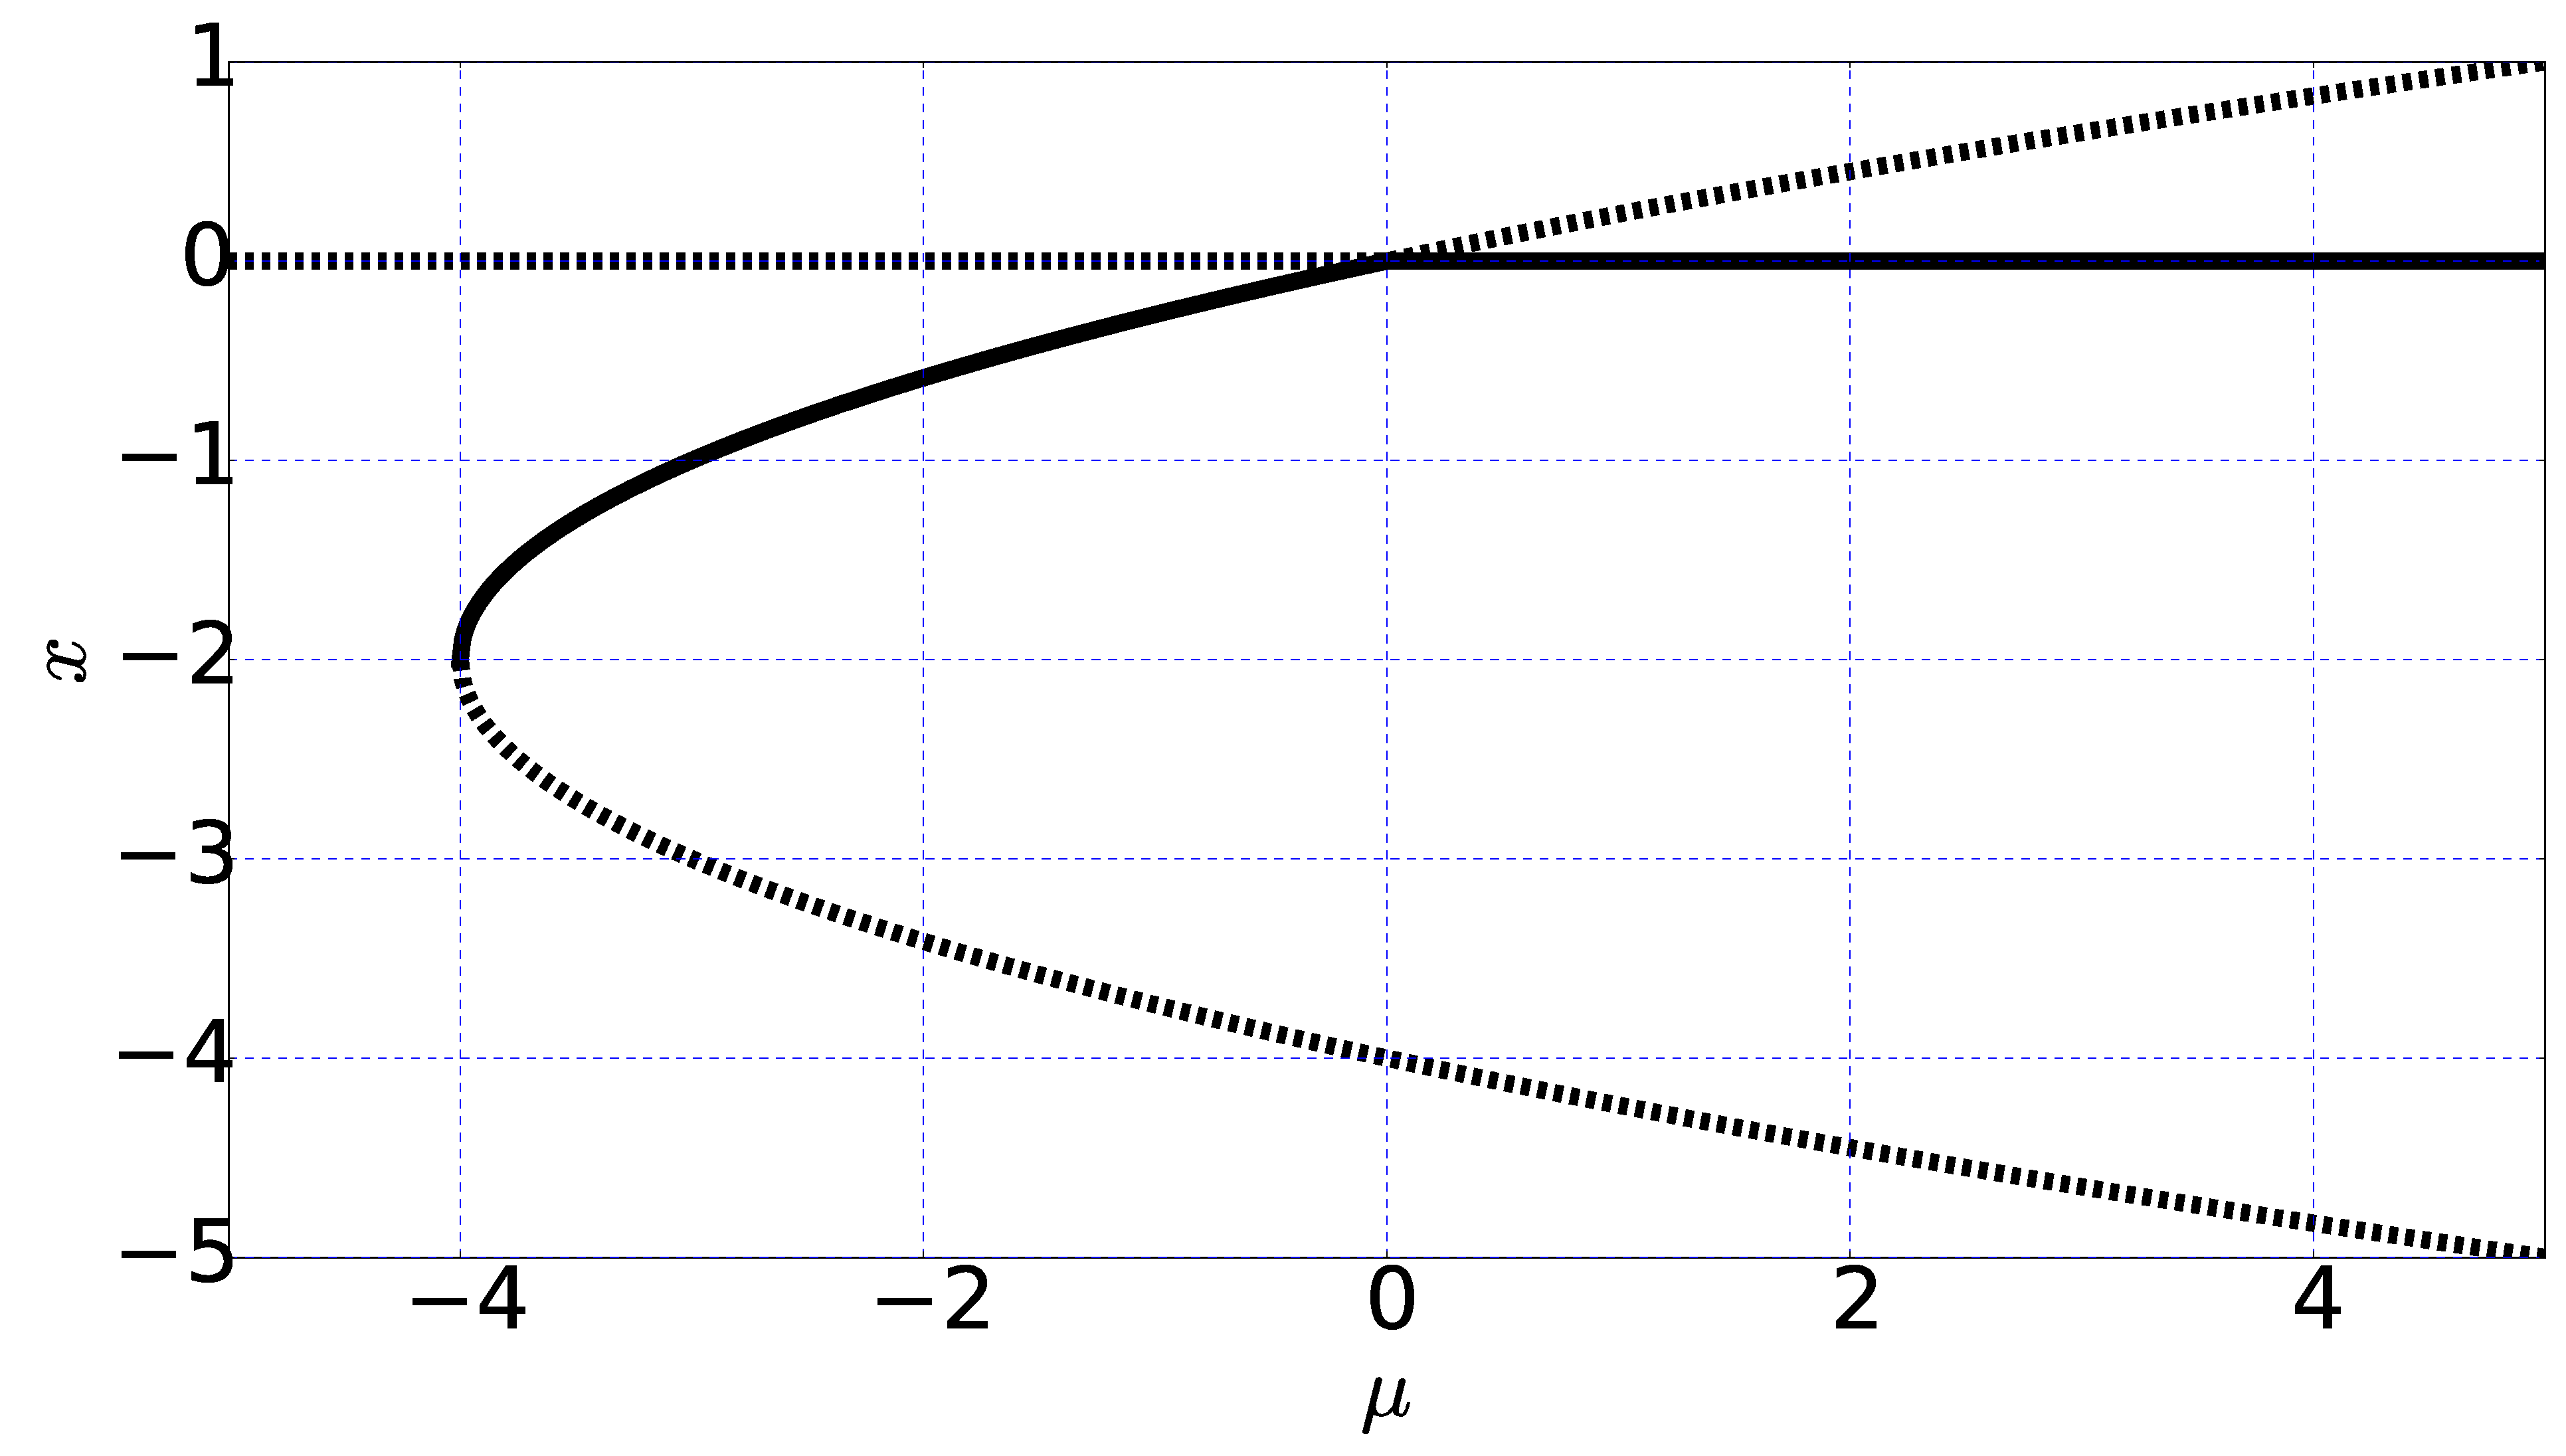
\includegraphics[width=8.0 cm]{figure/Q2/modified/delta4.eps}
		\caption{$\delta = 4$}
    \end{subfigure}
    \caption{Bifurcation diagram for different positive values for $\delta$. The dashed line is the \emph{unstable branch} and the solid line is the \emph{stable branch}.}
    \label{fig:bifurcation}
\end{figure}
%

For transcritical bifurcation, the number of stationary points for $\mu < 0$ and $\mu > 0$ remains the same (here 3) however, their characteristics change. Stable stationary points become unstable and unstable ones become stable. For small values of $\mu$, the pitchfork bifurcation at $(0, 0)$ can be considered a transcritical bifurcation for this reason. The bifurcation plots for small values of $x$ and $\delta$ are shown in Figure \ref{fig:bifurcationZoomed}.

%
\begin{figure}[h]
	\centering
	\begin{subfigure}[h]{8.0 cm}
		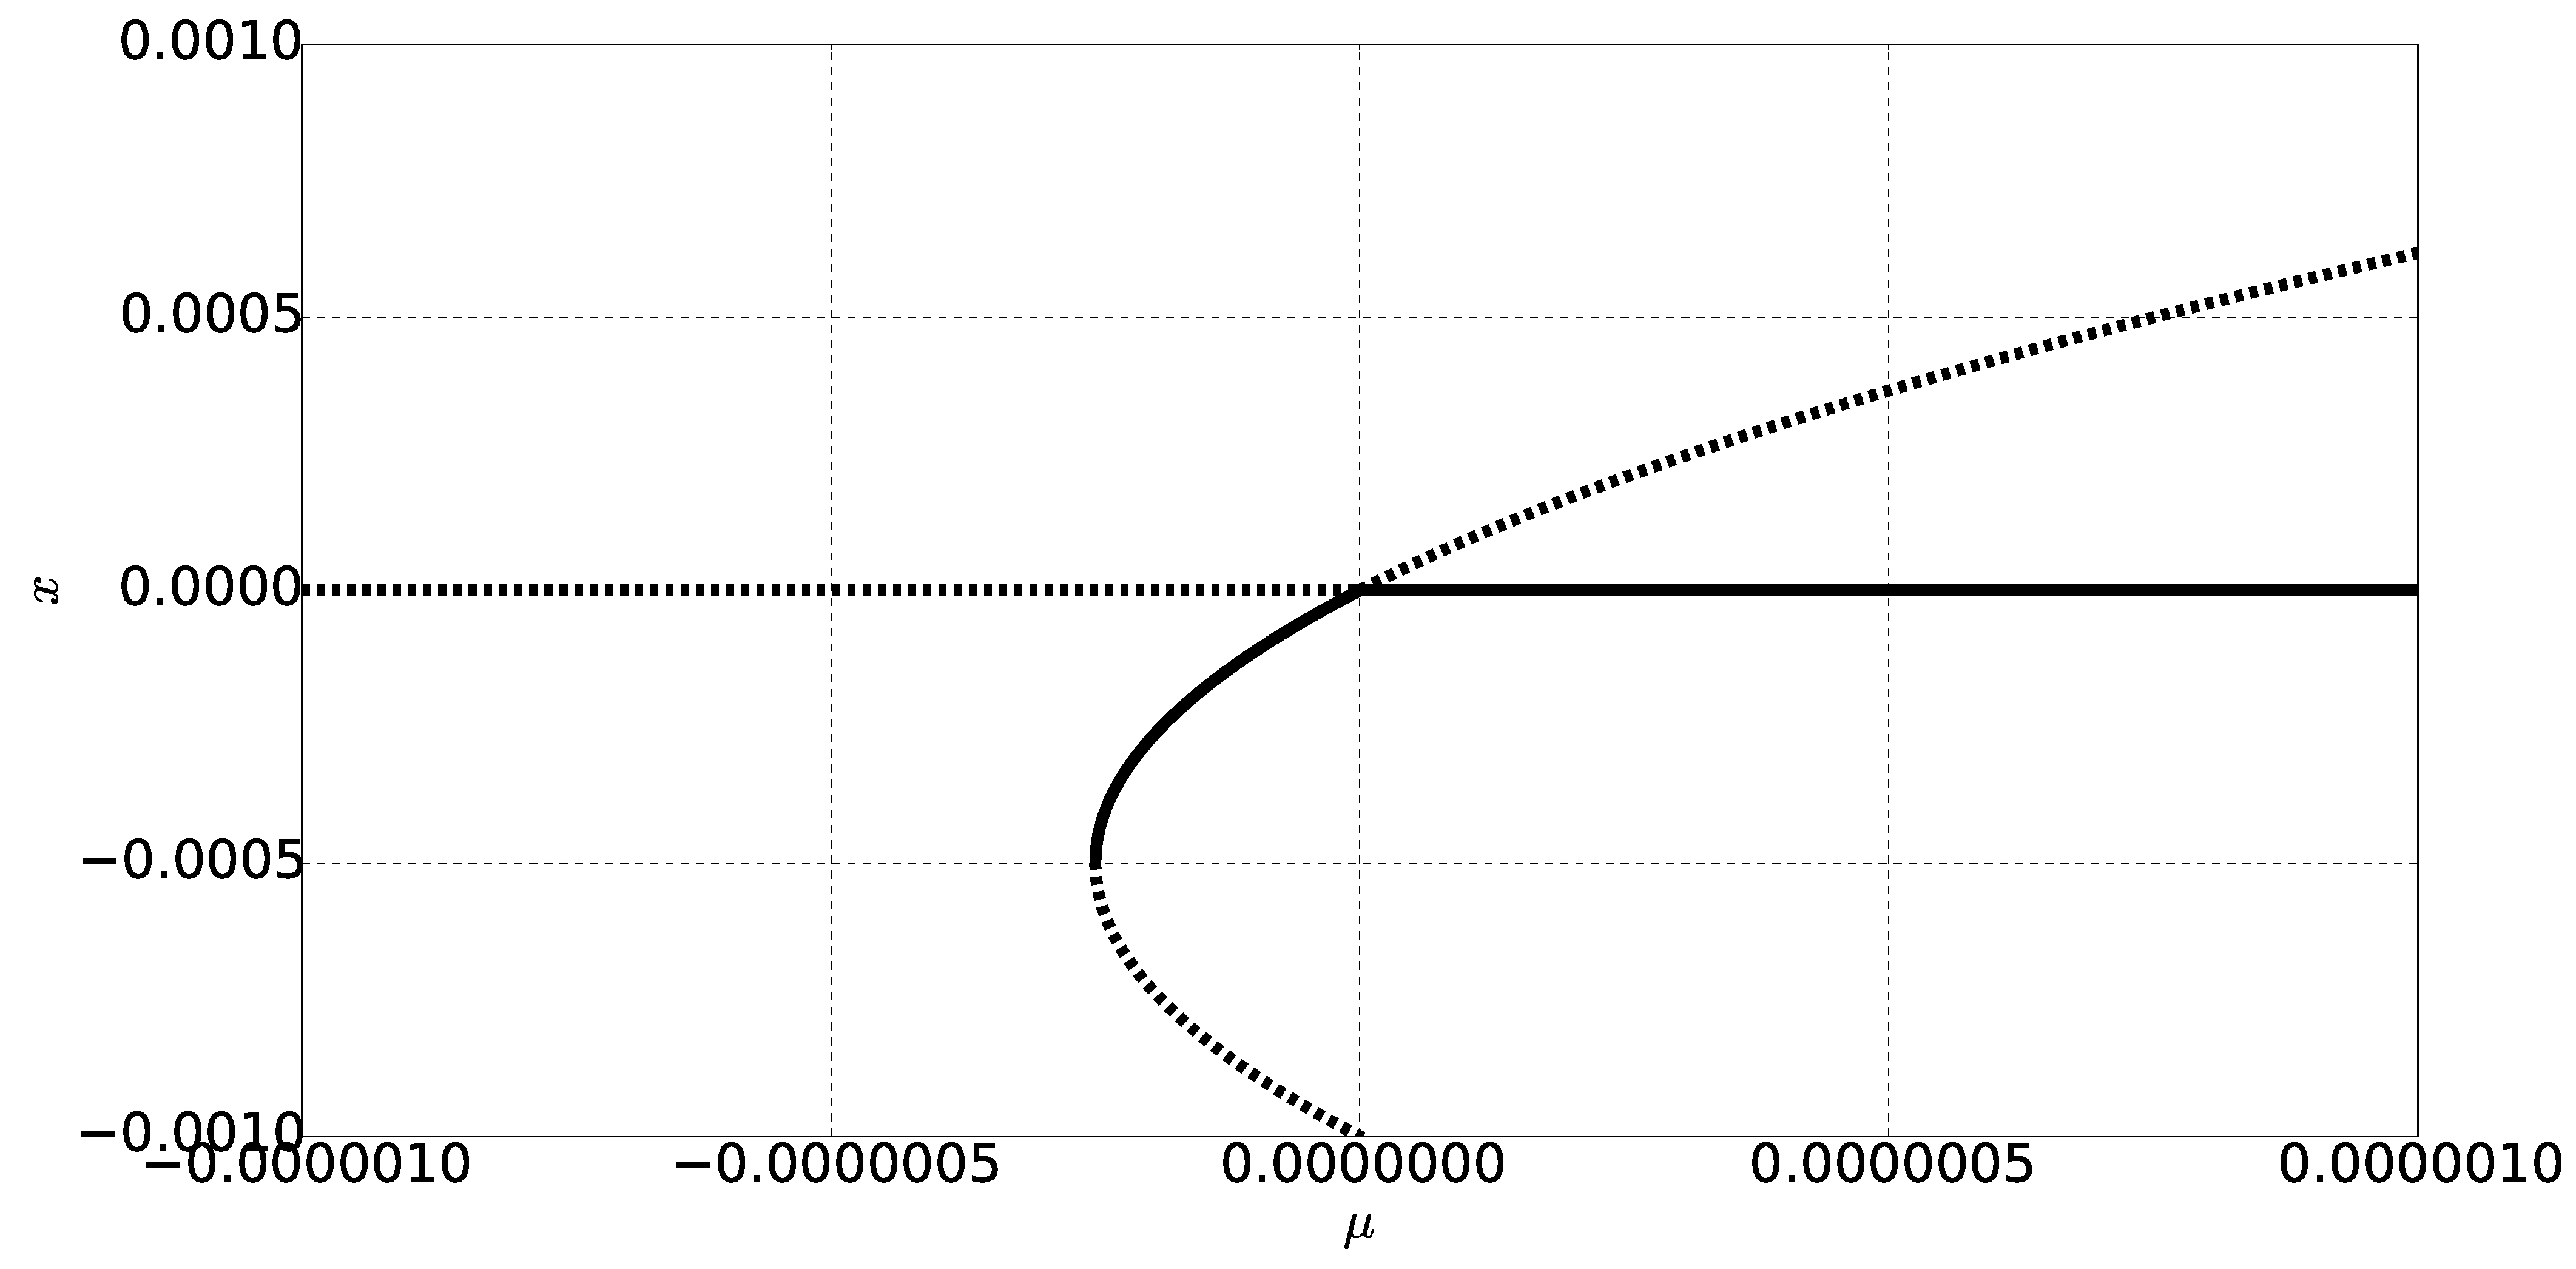
\includegraphics[width=8.0 cm]{figure/Q2/modified/delta0001_zoomed.eps}
		\caption{$\delta = 0.001$}
	\end{subfigure}
	\begin{subfigure}[h]{8.0 cm}
        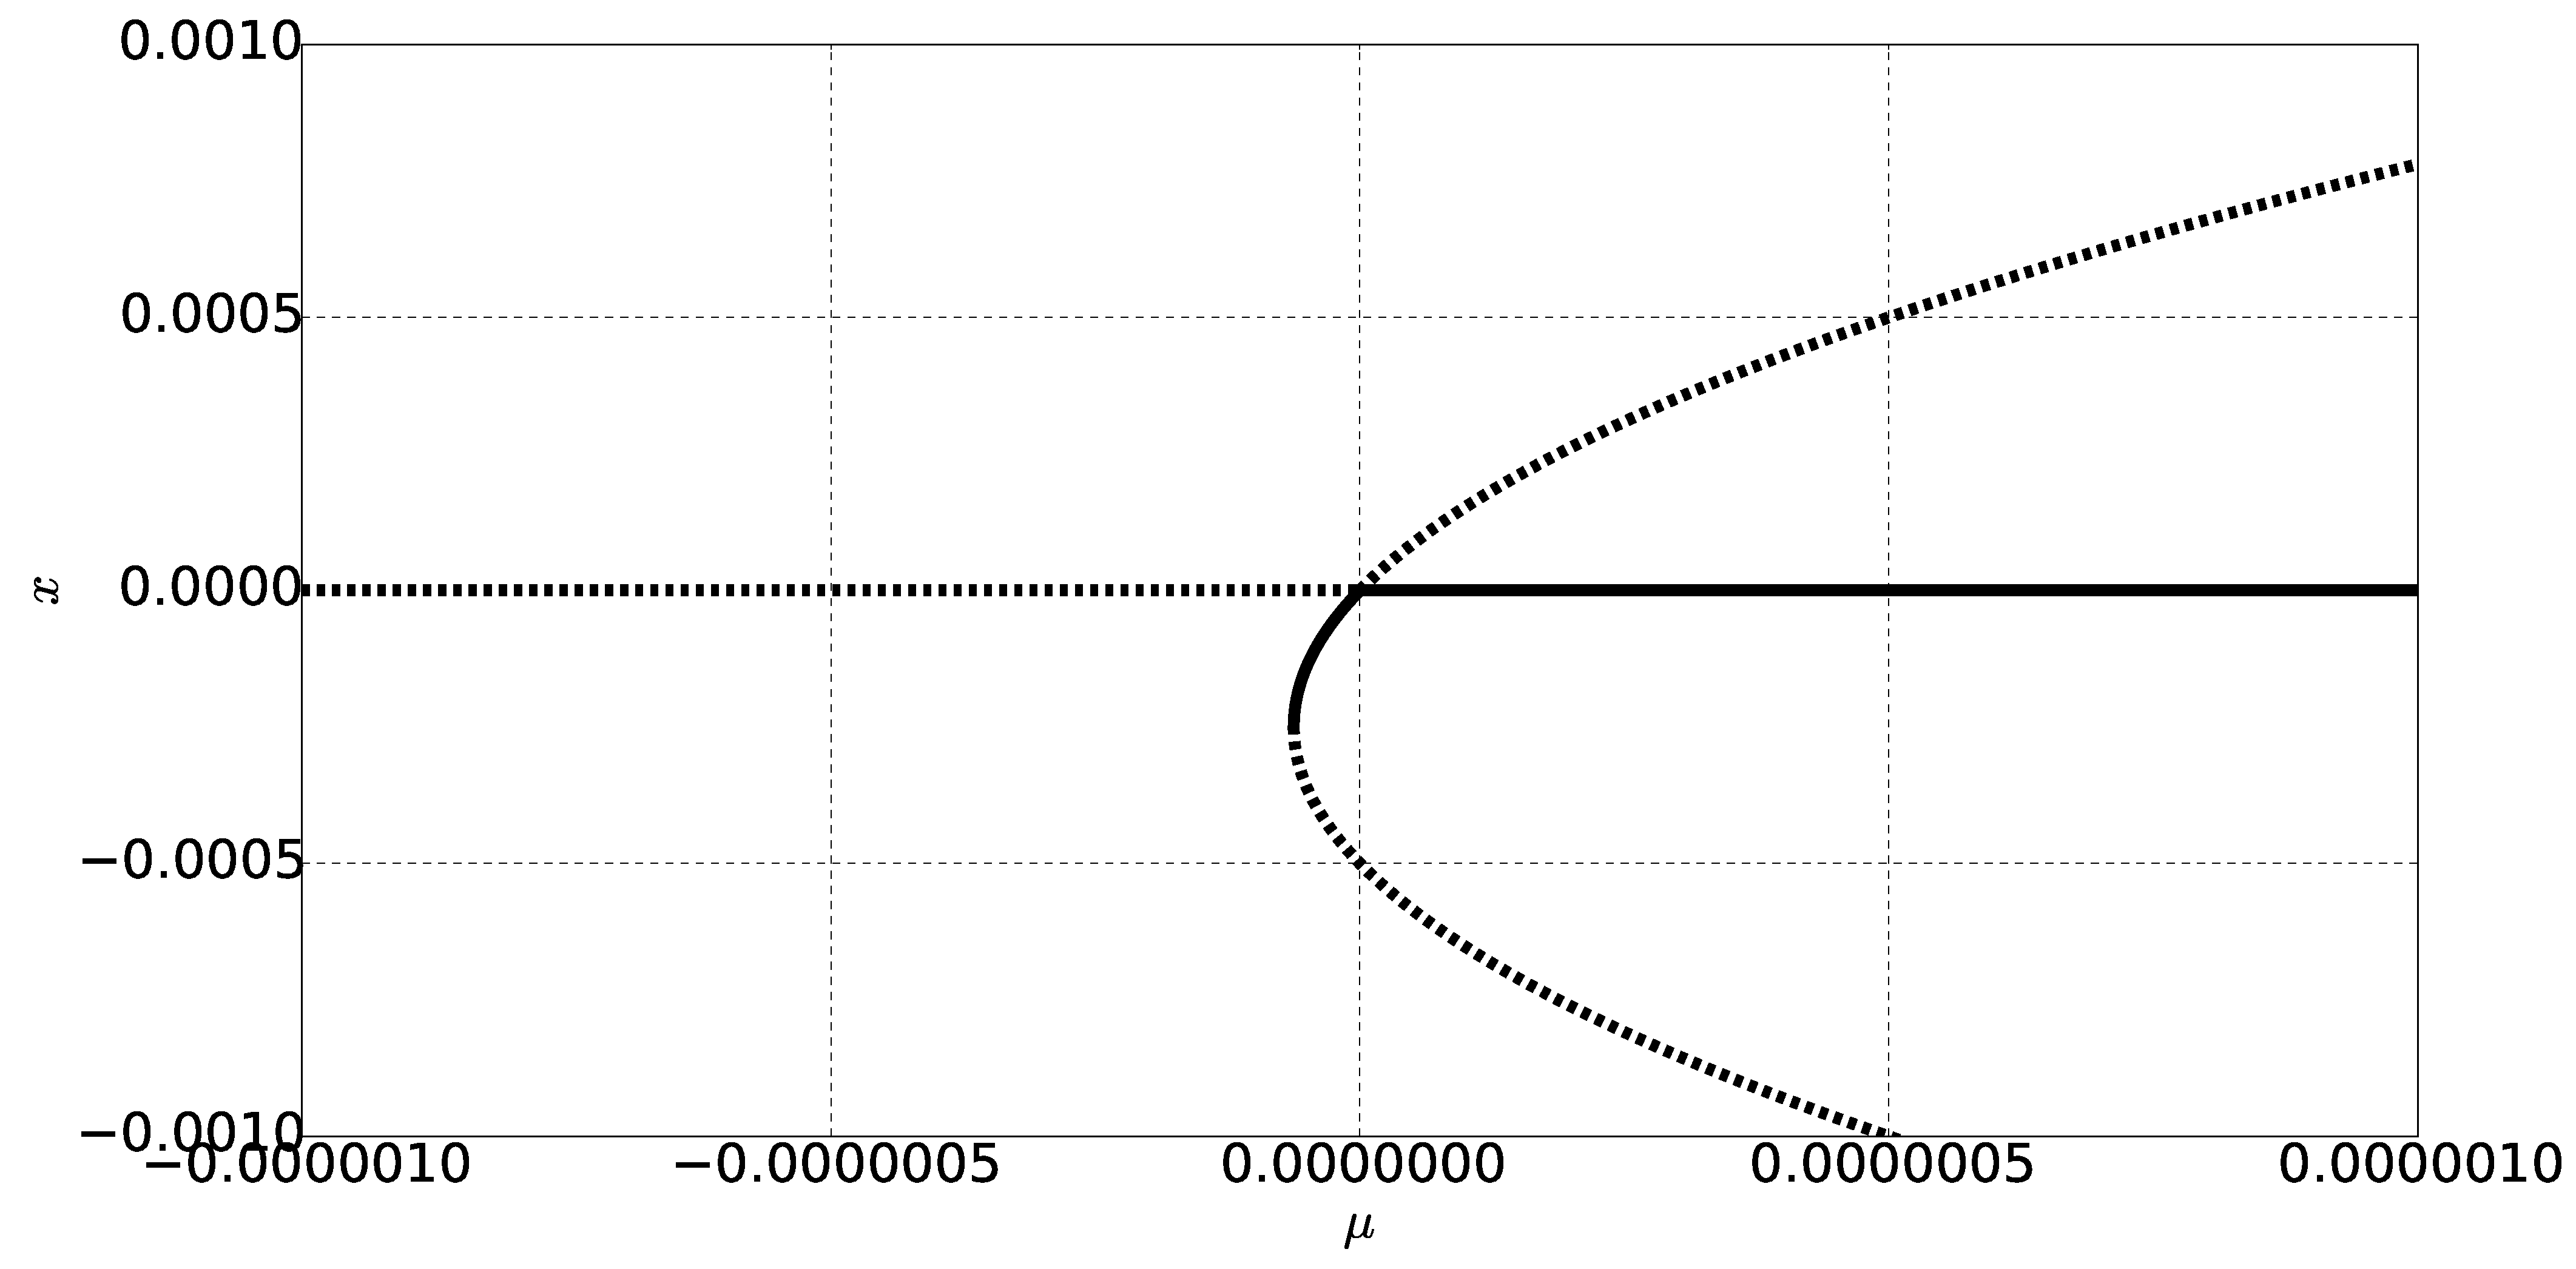
\includegraphics[width=8.0 cm]{figure/Q2/modified/delta00005_zoomed.eps}
		\caption{$\delta = 0.0005$}
    \end{subfigure}
    \caption{Bifurcation diagram for small values of $x$ and $\delta$. The dashed line is the \emph{unstable branch} and the solid line is the \emph{stable branch}.}
    \label{fig:bifurcationZoomed}
\end{figure}
%